\documentclass[11pt, letterpaper]{article}

\usepackage[margin=1in]{geometry}
\usepackage{booktabs}
\usepackage{enumitem}
\usepackage{tikz}
\usepackage{xcolor}
\usepackage{hyperref}
\usepackage{fancyhdr}
\usepackage{tabularx}

\usetikzlibrary{shapes.geometric, arrows.meta, positioning, fit, backgrounds, calc, decorations.pathreplacing}

% Colors
\definecolor{primary}{HTML}{2563EB}
\definecolor{secondary}{HTML}{7C3AED}
\definecolor{accent}{HTML}{059669}
\definecolor{warm}{HTML}{D97706}
\definecolor{lightbg}{HTML}{F1F5F9}
\definecolor{darktext}{HTML}{1E293B}
\definecolor{memcolor}{HTML}{7C3AED}
\definecolor{pipecolor}{HTML}{2563EB}
\definecolor{storecolor}{HTML}{059669}

\hypersetup{
    colorlinks=true,
    linkcolor=primary,
    urlcolor=primary,
}

\pagestyle{fancy}
\fancyhf{}
\rhead{Memory System Design}
\lhead{Conversation-to-Calendar AI}
\rfoot{Page \thepage}

\title{\textbf{Memory System Design}\\[0.3em]
\large Dual-Call Pipeline for Persistent Agent Memory\\
Conversation-to-Calendar AI}
\author{Capstone Project II}
\date{February 2026}

\begin{document}
\maketitle
\thispagestyle{fancy}

% ============================================================
\section{System Overview}

The memory system adds persistent state to the calendar AI pipeline using a
\textbf{dual-call architecture}: the main extraction LLM is augmented with memory
context (read path), and a separate post-processing LLM call extracts new memories
from each interaction (write path).

\begin{center}
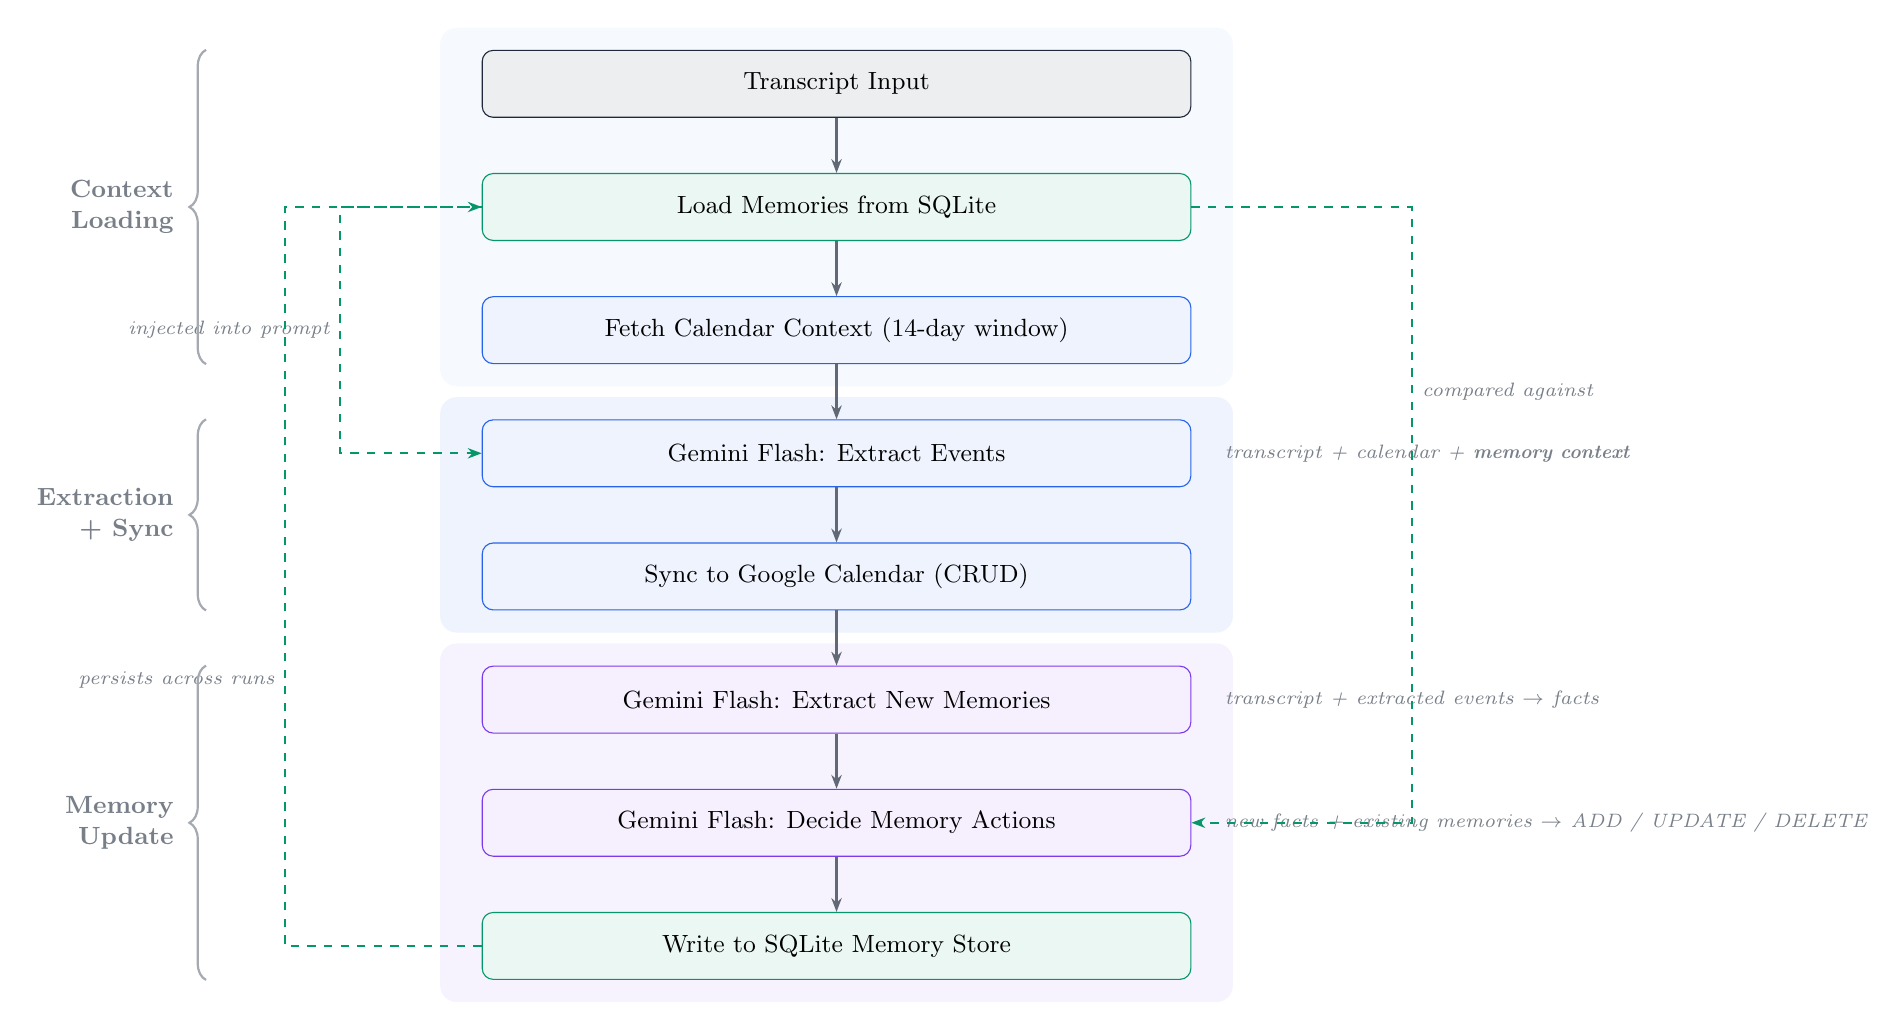
\begin{tikzpicture}[
    node distance=0.7cm,
    stage/.style={rectangle, draw=#1, fill=#1!8, rounded corners=4pt,
                  minimum width=9cm, minimum height=0.85cm, align=center,
                  font=\small},
    arrow/.style={-{Stealth[length=5pt]}, thick, color=darktext!70},
    note/.style={font=\scriptsize\itshape, text=darktext!60},
    mem/.style={rectangle, draw=memcolor, fill=memcolor!10, rounded corners=3pt,
                minimum width=3.2cm, minimum height=0.7cm, align=center,
                font=\small}
]

% Main pipeline stages
\node[stage=darktext] (input) {Transcript Input};
\node[stage=storecolor, below=of input] (loadmem) {Load Memories from SQLite};
\node[stage=pipecolor, below=of loadmem] (calcx) {Fetch Calendar Context (14-day window)};
\node[stage=pipecolor, below=of calcx] (extract) {Gemini Flash: Extract Events};
\node[note, right=0.3cm of extract] {transcript + calendar + \textbf{memory context}};
\node[stage=pipecolor, below=of extract] (sync) {Sync to Google Calendar (CRUD)};
\node[stage=memcolor, below=of sync] (memex) {Gemini Flash: Extract New Memories};
\node[note, right=0.3cm of memex] {transcript + extracted events $\rightarrow$ facts};
\node[stage=memcolor, below=of memex] (decide) {Gemini Flash: Decide Memory Actions};
\node[note, right=0.3cm of decide] {new facts + existing memories $\rightarrow$ ADD / UPDATE / DELETE};
\node[stage=storecolor, below=of decide] (write) {Write to SQLite Memory Store};

% Main flow arrows
\draw[arrow] (input) -- (loadmem);
\draw[arrow] (loadmem) -- (calcx);
\draw[arrow] (calcx) -- (extract);
\draw[arrow] (extract) -- (sync);
\draw[arrow] (sync) -- (memex);
\draw[arrow] (memex) -- (decide);
\draw[arrow] (decide) -- (write);

% Memory injection arrow (read path)
\draw[arrow, dashed, color=storecolor, thick]
    (loadmem.west) -- ++(-1.8,0) |- (extract.west)
    node[note, pos=0.25, left] {injected into prompt};

% Existing memory lookup arrow
\draw[arrow, dashed, color=storecolor, thick]
    (write.west) -- ++(-2.5,0) |- (loadmem.west)
    node[note, pos=0.18, left] {persists across runs};

% Existing memory fed to decision
\draw[arrow, dashed, color=storecolor]
    (loadmem.east) -- ++(2.8,0) |- (decide.east)
    node[note, pos=0.15, right] {compared against};

% Phase labels
\begin{scope}[on background layer]
    \node[fit=(input)(calcx), fill=pipecolor!4, rounded corners=6pt,
          inner xsep=15pt, inner ysep=8pt] {};
    \node[fit=(extract)(sync), fill=pipecolor!8, rounded corners=6pt,
          inner xsep=15pt, inner ysep=8pt] {};
    \node[fit=(memex)(write), fill=memcolor!6, rounded corners=6pt,
          inner xsep=15pt, inner ysep=8pt] {};
\end{scope}

% Phase annotations
\draw[decorate, decoration={brace, amplitude=6pt, mirror}, thick, darktext!40]
    ([xshift=-3.5cm]input.north west) -- ([xshift=-3.5cm]calcx.south west)
    node[midway, left=8pt, font=\small\bfseries, text=darktext!60, align=right] {Context\\Loading};

\draw[decorate, decoration={brace, amplitude=6pt, mirror}, thick, darktext!40]
    ([xshift=-3.5cm]extract.north west) -- ([xshift=-3.5cm]sync.south west)
    node[midway, left=8pt, font=\small\bfseries, text=darktext!60, align=right] {Extraction\\+ Sync};

\draw[decorate, decoration={brace, amplitude=6pt, mirror}, thick, darktext!40]
    ([xshift=-3.5cm]memex.north west) -- ([xshift=-3.5cm]write.south west)
    node[midway, left=8pt, font=\small\bfseries, text=darktext!60, align=right] {Memory\\Update};

\end{tikzpicture}
\end{center}

% ============================================================
\section{Read Path: Memory Injection into Extraction}

Before event extraction, all memories are loaded from SQLite and formatted as a
section in the system prompt---the same mechanism used for calendar context injection.

\subsection{Prompt Structure}

The extraction LLM's system prompt currently contains:

\begin{enumerate}[leftmargin=2em]
    \item Role \& perspective rules
    \item Filtering rules (what NOT to extract)
    \item CRUD decision rules (create / update / delete logic)
    \item Few-shot examples
    \item Output format specification
    \item \textbf{Your Calendar} --- 14-day event window with integer IDs
\end{enumerate}

\noindent Memory adds a 7th section:

\begin{quote}
\small
\texttt{\textbf{== Your Memory (learned from past conversations) ==}}\\[0.3em]
\texttt{\textbf{Preferences:}}\\
\texttt{- Alice prefers morning meetings (before 11am)}\\
\texttt{- Never schedule over lunch (12:00--1:00pm)}\\
\texttt{- Default meeting duration is 30 minutes}\\[0.3em]
\texttt{\textbf{People:}}\\
\texttt{- Bob is Alice's manager (weekly 1:1 on Tuesdays)}\\
\texttt{- Carol is on the design team}\\
\texttt{- Dave is an external client (meetings need formal titles)}\\[0.3em]
\texttt{\textbf{Vocabulary:}}\\
\texttt{- "quick sync" = 15 minutes}\\
\texttt{- "EOD" = 5:00pm}\\
\texttt{- "standup" = 15 minutes (corrected from 30)}\\[0.3em]
\texttt{\textbf{Patterns:}}\\
\texttt{- When Alice says "lunch meeting" she means 12:30pm}\\
\texttt{- Client meetings with Dave are usually 1 hour}
\end{quote}

\subsection{Why Full Injection Works}

At single-user scale, total memory will likely remain under 100 entries and
$\sim$2,000 tokens. Given Gemini Flash's 1M-token context window, this is negligible.
Full injection avoids the complexity of embedding-based retrieval and eliminates
the risk of missing relevant memories due to poor similarity matches.

\textbf{Important:} Gemini Flash exhibits context degradation after $\sim$20\%
window utilization. The combined calendar context ($\sim$500 tokens) + memory
context ($\sim$2,000 tokens) stays well under 1\% of the window.

\subsection{How Memory Influences Extraction}

\begin{table}[h]
\centering
\small
\begin{tabularx}{\textwidth}{XXX}
\toprule
\textbf{Transcript Says} & \textbf{Memory Provides} & \textbf{Result} \\
\midrule
``Set up a quick sync with Bob'' & ``quick sync = 15 min'' + ``Bob is Alice's manager'' & 15-min event, appropriate title \\
\addlinespace
``Lunch meeting tomorrow'' & ``lunch meetings = 12:30pm'' & Defaults to 12:30, not noon \\
\addlinespace
``Schedule standup for the team'' & ``standup = 15 min (corrected)'' & 15 min, not default 30 \\
\addlinespace
``Meeting with Dave next Tuesday'' & ``Dave = external client, usually 1hr'' & 1-hour event with formal title \\
\bottomrule
\end{tabularx}
\caption{Examples of memory-influenced extraction decisions.}
\end{table}

% ============================================================
\section{Write Path: Memory Extraction \& Update}

After event extraction and calendar sync, a separate pipeline extracts new memories
from the interaction and reconciles them with existing storage.

\subsection{Stage 1: Fact Extraction}

A dedicated Gemini Flash call receives the transcript and the extracted events,
then outputs candidate facts:

\begin{center}
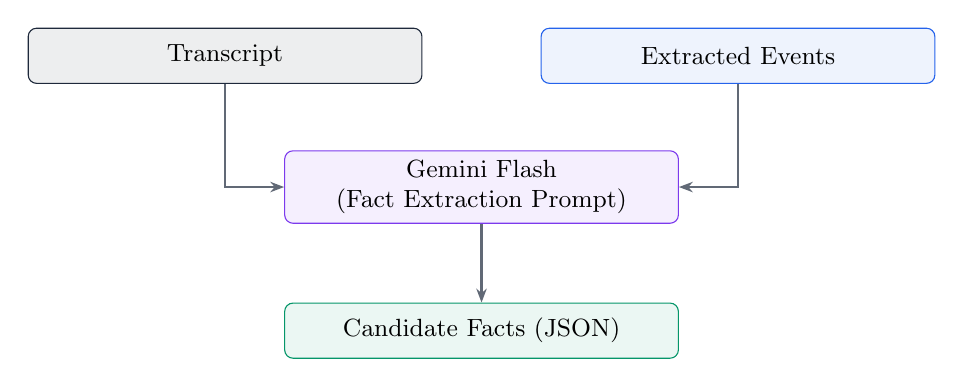
\begin{tikzpicture}[
    node distance=0.6cm,
    box/.style={rectangle, draw=#1, fill=#1!8, rounded corners=3pt,
                minimum width=5cm, minimum height=0.7cm, align=center,
                font=\small},
    arrow/.style={-{Stealth[length=5pt]}, thick, color=darktext!70}
]

\node[box=darktext] (in1) {Transcript};
\node[box=pipecolor, right=1.5cm of in1] (in2) {Extracted Events};
\node[box=memcolor, below=1.2cm of $(in1)!0.5!(in2)$] (llm) {Gemini Flash\\(Fact Extraction Prompt)};
\node[box=storecolor, below=1.0cm of llm] (out) {Candidate Facts (JSON)};

\draw[arrow] (in1) |- (llm);
\draw[arrow] (in2) |- (llm);
\draw[arrow] (llm) -- (out);

\end{tikzpicture}
\end{center}

\noindent The extraction prompt instructs the LLM to identify facts across categories:

\begin{itemize}[leftmargin=2em]
    \item \textbf{Preferences} --- scheduling habits, time-of-day patterns, duration defaults
    \item \textbf{People} --- names, relationships, roles, typical meeting patterns
    \item \textbf{Vocabulary} --- user-specific terms, abbreviations, implied durations
    \item \textbf{Corrections} --- when extracted events differ from user intent (if feedback available)
    \item \textbf{Patterns} --- recurring events, seasonal scheduling habits
\end{itemize}

\noindent Output format:
\begin{quote}
\small
\texttt{\{"facts": [}\\
\texttt{~~\{"category": "people", "key": "Bob",}\\
\texttt{~~~"value": "Alice's manager, weekly 1:1 on Tuesdays",}\\
\texttt{~~~"confidence": "high"\},}\\
\texttt{~~\{"category": "vocabulary", "key": "quick sync",}\\
\texttt{~~~"value": "15-minute meeting",}\\
\texttt{~~~"confidence": "medium"\}}\\
\texttt{]\}}
\end{quote}

\subsection{Stage 2: Memory Action Decision}

Each candidate fact is compared against existing memories. A second Gemini Flash call
decides the appropriate action:

\begin{center}
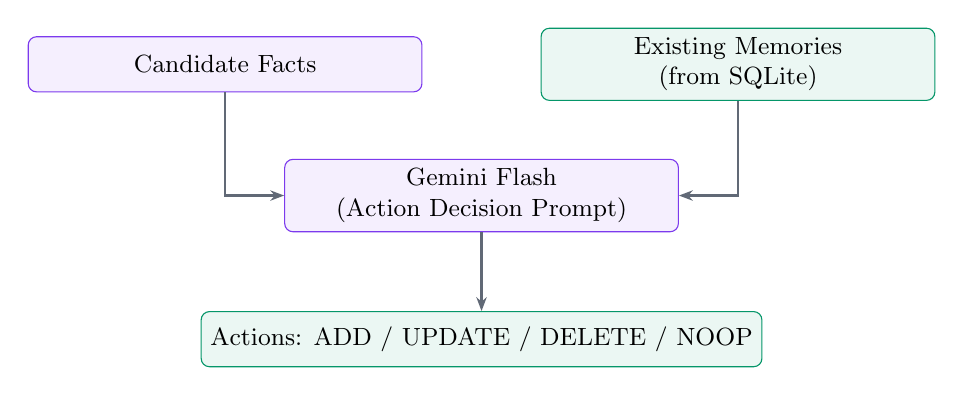
\begin{tikzpicture}[
    node distance=0.6cm,
    box/.style={rectangle, draw=#1, fill=#1!8, rounded corners=3pt,
                minimum width=5cm, minimum height=0.7cm, align=center,
                font=\small},
    arrow/.style={-{Stealth[length=5pt]}, thick, color=darktext!70}
]

\node[box=memcolor] (facts) {Candidate Facts};
\node[box=storecolor, right=1.5cm of facts] (existing) {Existing Memories\\(from SQLite)};
\node[box=memcolor, below=1.2cm of $(facts)!0.5!(existing)$] (llm) {Gemini Flash\\(Action Decision Prompt)};
\node[box=storecolor, below=1.0cm of llm] (actions) {Actions: ADD / UPDATE / DELETE / NOOP};

\draw[arrow] (facts) |- (llm);
\draw[arrow] (existing) |- (llm);
\draw[arrow] (llm) -- (actions);

\end{tikzpicture}
\end{center}

\noindent The decision prompt presents existing memories alongside new facts and asks
the LLM to choose:

\begin{table}[h]
\centering
\small
\begin{tabularx}{\textwidth}{lXX}
\toprule
\textbf{Action} & \textbf{When} & \textbf{Example} \\
\midrule
\textsc{add} & Genuinely new information & New person mentioned for the first time \\
\textsc{update} & Refines or contradicts existing memory & ``prefers mornings'' $\rightarrow$ ``prefers before 10am'' \\
\textsc{delete} & Information is no longer true & User explicitly says ``I no longer work with Bob'' \\
\textsc{noop} & Already known or not worth storing & Duplicate or trivial fact \\
\bottomrule
\end{tabularx}
\caption{Memory action decision logic.}
\end{table}

\noindent\textbf{Key design choice:} The LLM makes the semantic decision, not a
similarity threshold. Only an LLM can distinguish supplementary information
(``prefers mornings'' + ``likes 9am slots'' $\rightarrow$ merge) from contradictory
information (``prefers mornings'' + ``switched to afternoons'' $\rightarrow$ replace).

\textbf{Optimization:} Stages 1 and 2 can be collapsed into a single LLM call that
receives the transcript, extracted events, \emph{and} existing memories, then outputs
actions directly. This trades some separation of concerns for lower latency and cost.

% ============================================================
\section{Storage: SQLite Schema}

\begin{quote}
\small
\begin{verbatim}
CREATE TABLE memories (
    id          INTEGER PRIMARY KEY AUTOINCREMENT,
    category    TEXT NOT NULL,       -- preferences | people | vocabulary | patterns | corrections
    key         TEXT NOT NULL,       -- lookup identifier (e.g., person name, term)
    value       TEXT NOT NULL,       -- the actual memory content
    confidence  TEXT DEFAULT 'medium', -- low | medium | high
    source_count INTEGER DEFAULT 1, -- # conversations confirming this fact
    created_at  TEXT NOT NULL,       -- ISO 8601
    updated_at  TEXT NOT NULL,       -- ISO 8601
    UNIQUE(category, key)           -- natural dedup within category
);

CREATE TABLE memory_log (
    id          INTEGER PRIMARY KEY AUTOINCREMENT,
    memory_id   INTEGER,            -- FK to memories (NULL for ADD before insert)
    action      TEXT NOT NULL,       -- ADD | UPDATE | DELETE | NOOP
    old_value   TEXT,               -- previous value (for UPDATE/DELETE)
    new_value   TEXT,               -- new value (for ADD/UPDATE)
    transcript  TEXT,               -- source transcript filename
    created_at  TEXT NOT NULL
);
\end{verbatim}
\end{quote}

\noindent Design notes:

\begin{itemize}[leftmargin=2em]
    \item \textbf{UNIQUE(category, key)} enforces natural deduplication---the LLM's
          \textsc{update} action maps to an \texttt{INSERT OR REPLACE}.
    \item \textbf{source\_count} increments when a fact is confirmed across multiple
          conversations, providing implicit confidence boosting.
    \item \textbf{memory\_log} provides a full audit trail of every memory change,
          supporting the demo requirement for observable AI reasoning.
    \item No vector embeddings or external dependencies---SQLite is in Python's standard library.
\end{itemize}

% ============================================================
\section{Memory Categories}

\begin{table}[h]
\centering
\small
\begin{tabularx}{\textwidth}{llX}
\toprule
\textbf{Category} & \textbf{Key Example} & \textbf{Value Example} \\
\midrule
\texttt{preferences} & \texttt{meeting\_time} & Alice prefers morning meetings (before 11am) \\
\texttt{preferences} & \texttt{lunch\_block} & Never schedule over lunch (12:00--1:00pm) \\
\texttt{people} & \texttt{Bob} & Alice's manager; weekly 1:1 on Tuesdays \\
\texttt{people} & \texttt{Dave} & External client; meetings need formal titles, usually 1hr \\
\texttt{vocabulary} & \texttt{quick sync} & 15-minute meeting \\
\texttt{vocabulary} & \texttt{EOD} & 5:00pm Pacific \\
\texttt{patterns} & \texttt{lunch\_meeting} & When Alice says ``lunch meeting'' she means 12:30pm \\
\texttt{corrections} & \texttt{standup\_duration} & Standup is 15 min, not 30 (corrected 2026-02-20) \\
\bottomrule
\end{tabularx}
\caption{Memory categories with representative entries.}
\end{table}

% ============================================================
\section{Cost Analysis}

\begin{table}[h]
\centering
\begin{tabularx}{\textwidth}{Xrrr}
\toprule
\textbf{LLM Call} & \textbf{Input (est.)} & \textbf{Output (est.)} & \textbf{Cost (est.)} \\
\midrule
Event extraction (existing) & $\sim$4,000 tokens & $\sim$500 tokens & \$0.010 \\
Memory extraction (new) & $\sim$3,000 tokens & $\sim$300 tokens & \$0.007 \\
Memory action decision (new) & $\sim$2,000 tokens & $\sim$200 tokens & \$0.005 \\
\midrule
\textbf{Total per pipeline run} & & & \textbf{$\sim$\$0.022} \\
\bottomrule
\end{tabularx}
\caption{Estimated cost per pipeline run using Gemini 2.5 Flash pricing
(\$0.15/1M input, \$3.50/1M output --- thinking off).}
\end{table}

\noindent The memory system adds approximately \$0.012 per run---roughly doubling
the per-run LLM cost, but remaining negligible in absolute terms.

% ============================================================
\section{Integration Points}

The memory system touches the following existing modules:

\begin{table}[h]
\centering
\small
\begin{tabularx}{\textwidth}{llX}
\toprule
\textbf{File} & \textbf{Change} & \textbf{Description} \\
\midrule
\texttt{prompts.py} & Modify & Add ``Your Memory'' section to system prompt builder \\
\texttt{pipeline.py} & Modify & Add memory load (before extraction) and memory update (after sync) stages \\
\texttt{llm.py} & Modify & Accept \texttt{memory\_context} parameter in \texttt{extract\_events()} \\
\texttt{memory/} & \textbf{New} & New subpackage: store, extraction, prompts \\
\texttt{config.py} & Modify & Add memory DB path to Settings \\
\bottomrule
\end{tabularx}
\caption{Files affected by memory system integration.}
\end{table}

\end{document}
